%%%%%%%%%%%% DOCUMENT BEGINS %%%%%%%%%%%%%%%%%%%%%
\input{tutorial-preamble.tex}

\usepackage{subcaption}
\captionsetup{compatibility=false}


\author{Department of Aeronautics, Imperial College London, UK\newline
Scientific Computing and Imaging Institute, University of Utah, USA}
\title{Quasi-3D Computation of the Taylor-Green Vortex Flow}
\date{\today}

\begin{document}

% Render pretty title page if not building HTML
\ifdefined\HCode
\begin{center}
    \includegraphics[width=0.1\textwidth]{img/icon-blue.png}
\end{center}
\maketitle
\begin{center}
    \huge{Tutorials}
\end{center}
\else
\titlepage
\fi

\clearpage

\chapter{Introduction}
This tutorial describes the use of the spectral/\textit{$hp$} element
framework \textit{Nektar++} to explore one of the classical and canonical problems of fluid dynamics: the Taylor-Green Vortex (TGV). Information on how to install the libraries, solvers, and utilities on your own computer is available on the webpage \href{http://www.nektar.info}{\underline{www.nektar.info}}.

\begin{tutorialtask}
Prepare for the tutorial. Make sure that you have:
\begin{itemize}
  \item Installed and tested \nektar v\nekver~from a binary package, or
      compiled it from source. Note that sources may be compiled with the
	  CMake options \inltt{NEKTAR\_USE\_FFTW} and \inltt{NEKTAR\_USE\_MPI}
	  set to \texttt{ON} for faster execution. By default
	  binary packages will install all executables in
      \inlsh{/usr/bin}. If you compile from source they will be in the
      sub-directory \inlsh{dist/bin} of the \inlsh{build} directory you
      created in the \nektar source tree. We will refer to the directory
      containing the executables as \inlsh{\$NEK} for the remainder of the
      tutorial.
   \item Downloaded the tutorial files: 
       \relurl{incns-taylor-green-vortex.tar.gz}{incns-taylor-green-vortex}\\
   Unpack it using
   \inlsh{unzip incns-taylor-green-vortex.tar.gz}
   to produce a directory \inlsh{incns-taylor-green-vortex} with subdirectories
        called \inlsh{tutorial} and \inlsh{complete}.
   We will refer to the \inlsh{tutorial} directory as \inlsh{\$NEKTUTORIAL}. 
\end{itemize}
\end{tutorialtask}


\noindent
The TGV flow case has analytical initial conditions and its exact
solution is known from direct numerical simulation (DNS) using
incompressible Navier-Stokes solvers. For this reason it is often used for
code validation. Moreover, the TGV flow problem is a very instructive analysis
case: through its numerical simulation, it is possible to study turbulent
transition and decay, vortex dynamics and energy dissipation mechanisms
\footnote{G.I.~Taylor and A.E.~Green.\newblock{Mechanism of the Production of
Small Eddies from Large Ones}.\newblock{\em Proceedings of the Royal Society A:
Mathematical, Physical and Engineering Sciences}, 158:499--521, 1937.}. In this
tutorial we will focus on the solution of the TGV flow case in a 3D cube region
within a time frame of 20 seconds, which is usually sufficient to observe the
aforementioned phenomena. For now, we will restrict ourselves to a resolution of
$64^{3}$ degrees of freedom using $p=8$ order interpolants in a
Continuous Galerkin (CG) projection. We will also have a look at the temporal
evolution of the kinetic enery and its dissipation rate in the flow domain.
The case with $128^{3}$ degrees of freedom is left as an optional exercise for the user.
 

The necessary files to complete this tutorial are included in the .zip folder downloaded using the link in \texttt{Task 1.1}. Under the folder \texttt{tutorial}, the user will find four subfolders, two for each resolution (64 or 128):


\begin{itemize}
\item Folder \texttt{geometry64}
\begin{itemize}
\item \texttt{TGV64\_mesh.msh} - \gmsh generated mesh data listing mesh vertices and elements for the $64^{3}$ case.
\end{itemize}
\end{itemize}

\begin{itemize}
\item Folder \texttt{geometry128}
\begin{itemize}
\item \texttt{TGV128\_mesh.msh} - \gmsh generated mesh data listing mesh vertices and elements for the $128^{3}$ case.
\end{itemize}
\end{itemize}

\begin{itemize}
\item Folder \texttt{solver64}
\begin{itemize}
\item \texttt{TGV64\_mesh.xml} - \nektar session file, generated with the
\texttt{\$NEK/NekMesh} utility, containing the 2D mesh for the $64^{3}$ case.
\item \texttt{TGV64\_conditions.xml} - \nektar session file containing the solver settings for the $64^{3}$ case.
\item \texttt{shell64.sh} - A bash script with the required command structure to automatically run the simulation on the compute nodes at Imperial College London.
\end{itemize}
\end{itemize}

\begin{itemize}
\item Folder \texttt{solver128}
\begin{itemize}
\item \texttt{TGV128\_mesh.xml} - \nektar session file, generated with the
\texttt{\$NEK/NekMesh} utility, containing the 2D mesh for the $128^{3}$ case.
\item \texttt{TGV128\_conditions.xml} - \nektar session file containing the solver settings for the $128^{3}$ case.
\item \texttt{shell128.sh} - A bash script with the required command structure to automatically run the simulation on the compute nodes at Imperial College London.
\end{itemize}
\end{itemize}

The folder \texttt{completed} that can also be found in the \texttt{.zip} contains the filled \texttt{.xml} files to be used as a check in case the user gets stuck, or to verify the correctness at the end of the tutorial.

\begin{tipbox}

Because the test case can take some time to complete, you may want to run the solver
with the completed configurations files available in the folder \texttt{completed}.
To do so, in the folder \texttt{completed/solver64}, type the following command on the
command line:
\tutorialcommand{\$NEK/IncNavierStokesSolver TGV64\_mesh.xml TGV64\_conditions.xml}

Note that this is entirely optional as output files are already provided in the same
folder, i.e. \texttt{completed/solver64}.

\end{tipbox}

\chapter{Background}
The TGV is an exact solution of the incompressible Navier-Stokes equations: 


\begin{align*}
\frac{\partial \textbf{V}}{\partial t} + \textbf{V} \cdot \nabla
    \textbf{V}&=-\nabla P+ \nu \nabla^{2}\textbf{V},\\
    \nabla \cdot \textbf{V}&=0,
\end{align*}

\noindent 
where $\textbf{V}=(u,v,w)$ is the velocity of the fluid in the x, y and z directions respectively, $P$ is the pressure, $\rho$ is the density and $\nu$ is the kinematic viscosity. Note that the absence of a forcing function (body force) will result in viscosity dissipating all the energy in the fluid, which will then eventually come to rest.

\noindent
In order to simulate the flow, the Velocity Correction Scheme will be used to evaluate the Navier-Stokes equations. This scheme uses a projection in which the velocity matrix and pressure are decoupled. For detailed information on the method, you can consult the \href{http://www.nektar.info/downloads/8/}{User-Guide}. 

\section*{Quasi-3D Approach}
Instead of constructing a 3D mesh of the domain and applying a spectral/\textit{$hp$}
discretisation in all three directions, it is more computationally efficient to
use a quasi-3D approach. This approach allows the use of a spectral/\textit{$hp$}
expansion on a 2D mesh and to extend the computation in the third direction
(typically the z-direction) using a simpler purely spectral harmonic
discretisation (classically a Fourier expansion), if that direction is geometrically homogeneous.
The user needs only specify the number of modes and basis type for the
discretisation and the length along the z-direction.

\section*{Mesh and Boundary Conditions}
The mesh we will use for the TGV flow is periodic in nature. It
is therefore defined as $-\pi L \leq x,y,z \leq \pi L$, where $L$ is the
inverse of the wavenumber of the minimum frequency that can be captured on our
mesh, i.e the largest length scale of our flow, known as the integral scale. It
represents the size of the large, energy-carrying eddies responsible for most of
the momentum transport. Given that the smallest length scale we can capture on
our mesh $\Delta x=\left(2\pi L/N\right)_{1D}$ in one direction, it is clear
that decreasing the integral scale $L$ (for a periodic mesh, by decreasing its size) or increasing the number of mesh points $N$, allows us to capture smaller and smaller flow scales.

\noindent
Since the TGV flow transitions to turbulence at a certain time, we would hope to capture the smallest turbulent length scales with our mesh. The smallest length scale $\eta$ in one direction, as defined by Kolgomorov is:

\begin{equation}
\frac{\eta}{L}\approx Re^{-3/4}
\end{equation}

\noindent
Then the number of points required for a homogeneous mesh in 3D to capture the Kolgomorov scales is (with $L=\mathcal{O}(1)$):

\begin{equation}
N_{3D}=\left(\frac{L}{\eta}\right)^{3}=\left(Re^{3/4}\right)^{3}=Re^{9/4}
\end{equation}

\noindent
Thus, for flow simulations of the TGV, which are usually run at $Re=1600$, the
number of uniform mesh points required to capture the smallest turbulent length
scales is $16,190,861$. The discretisation used in the current tutorial of
$N_{3D}=64^{3}=262,144$ points does not have enough resolution to resolve these
scales, and neither does the case with $N_{3D}=128^{3}=2,097,152$ points, left
as an exercise. The case with  $N_{3D}=256^{3}=16,777,216$ points would be
sufficient but to simulate the flow with such a fine mesh requires the aid of a
larger parallel computer, given the much larger memory requirements of the
computation. When the flow is underresolved some stabilisation is typically
required and this is why we will use a technique known as spectral vanishing
viscosity for the lower resolution runs.


\noindent
As mentioned above, the mesh used in this tutorial is a uniform square mesh of
length $-\pi \leq x,y \leq \pi $ ($L=1$) containing $64$ square elements, each
with a spectral/\textit{$hp$} expansion basis of order 8.
This 2D mesh is then expanded in the z-direction to compute the quasi-3D flow.
The homogeneous z-direction will be discretised using 64 planes. Boundary and
initial conditions are also applied. The latter will be described in the
following section. As for the former, given the periodic nature of the flow,
periodic boundary conditions are applied on all edges of the mesh. The 2D
meshes $64$ and $128$, showing all quadrature points, are shown in Fig.~\ref{f:mesh}:

\begin{figure}[h!]
 \centering
       \includegraphics[width=0.65\linewidth]{img/grid64.eps}\\
       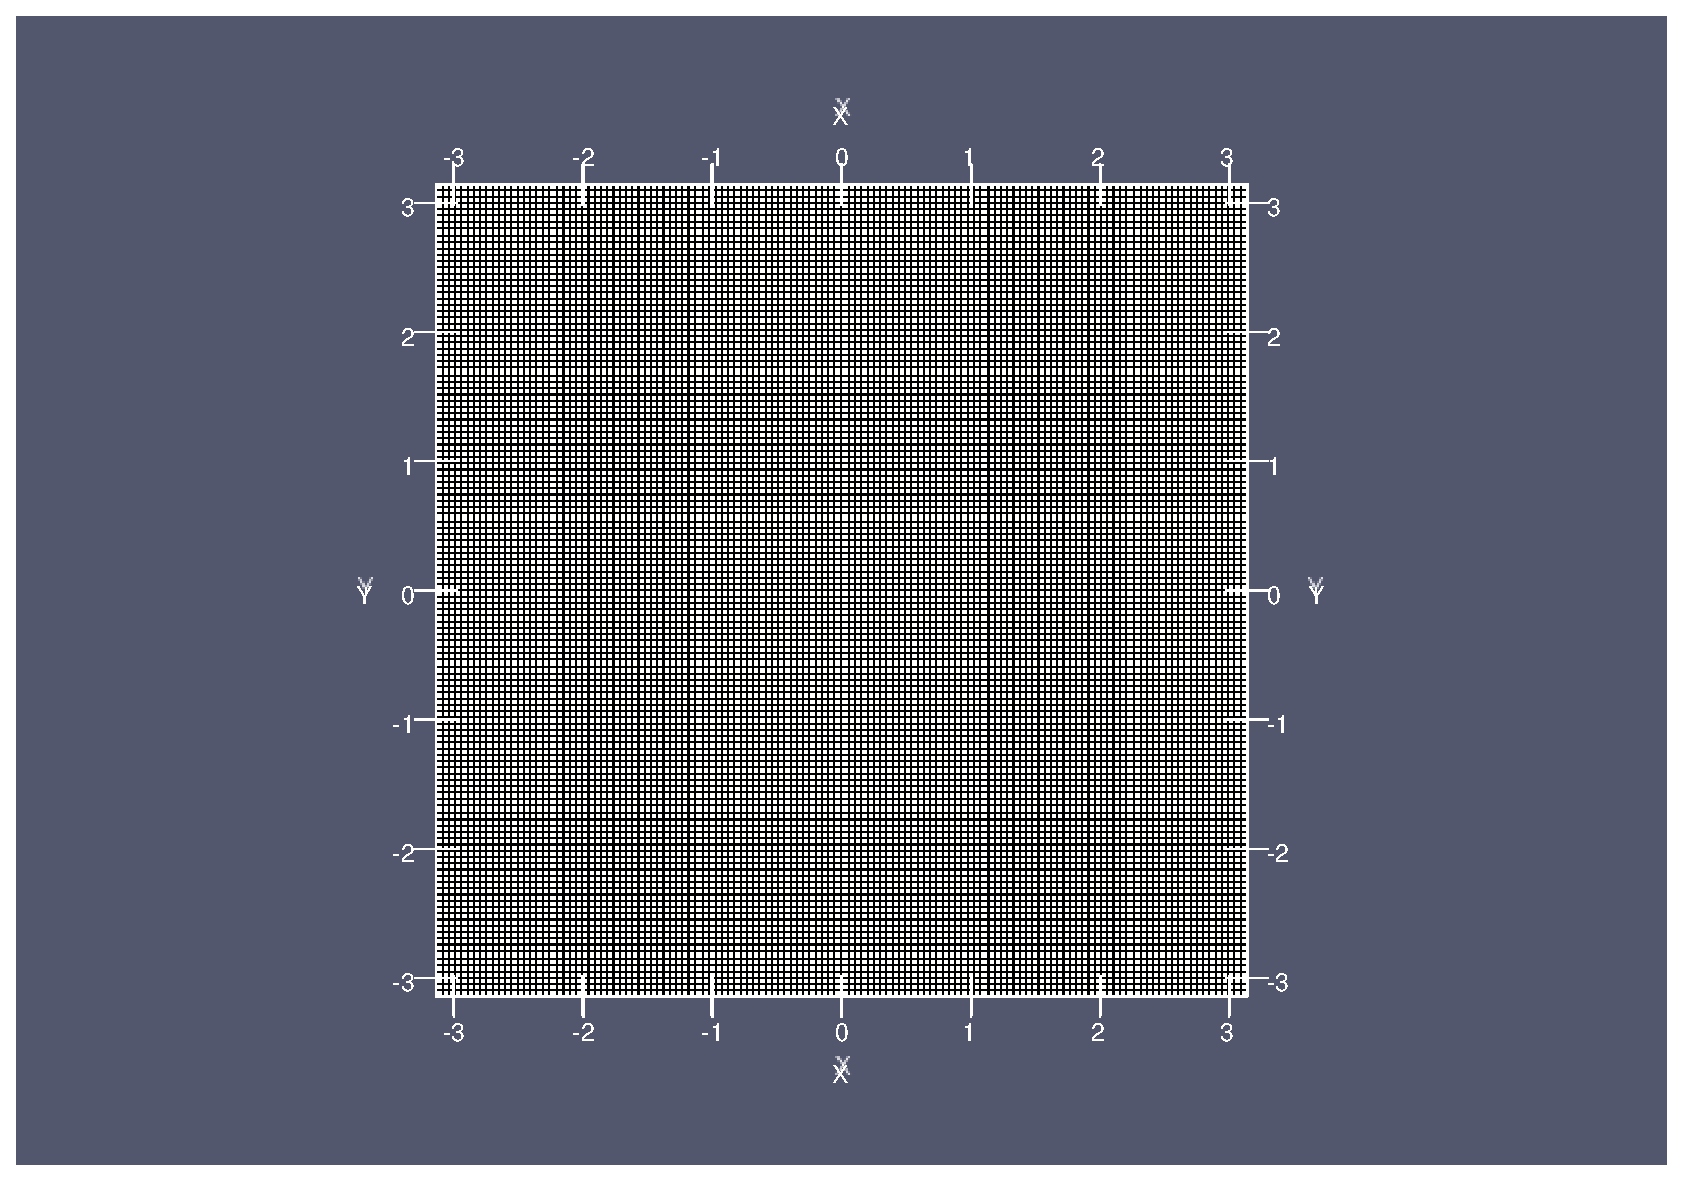
\includegraphics[width=0.65\linewidth]{img/grid128.eps}\\
       \caption{$64^{2}$ and $128^{2}$ element meshes.}
       \label{f:mesh}
\end{figure}

\vspace{5 cm}

\subsubsection*{Initial Conditions}
We are solving an initial value problem and in order to march the problem
forward in time we need to prescribe initial conditions for all variables. For
this case the initial conditions correspond to the TGV flow, given by:

\begin{align*}
    u(x,y,z, t=0)&=V_{0}\sin \left(\frac{x}{L}\right)\cos
    \left(\frac{y}{L}\right)\cos \left(\frac{z}{L}\right),\\
    v(x,y,z, t=0)&=-V_{0}\cos \left(\frac{x}{L}\right)\sin
    \left(\frac{y}{L}\right)\cos \left(\frac{z}{L}\right)\\\
    w(x,y,z, t=0)&=0,\\
    P(x,y,z, t=0)&=0.
\end{align*}


\begin{figure}
 \centering
       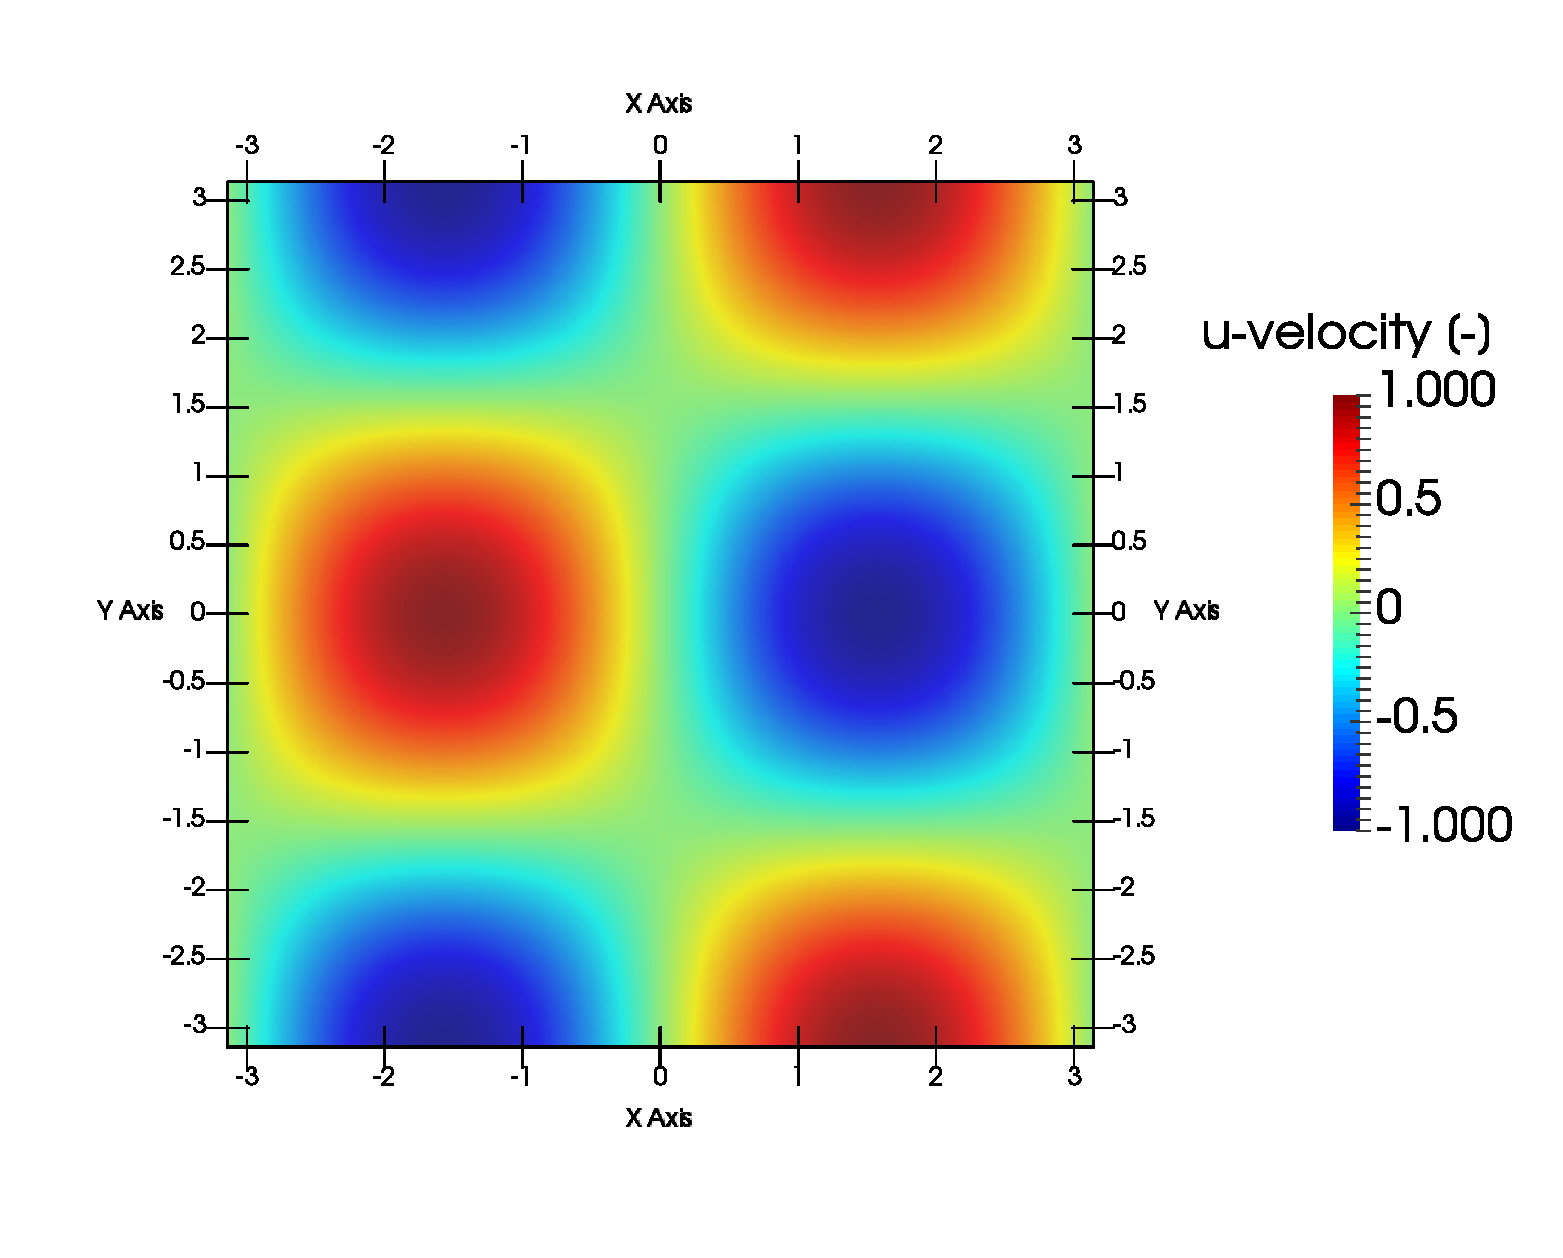
\includegraphics[width=0.48\linewidth]{img/ufield.eps}
       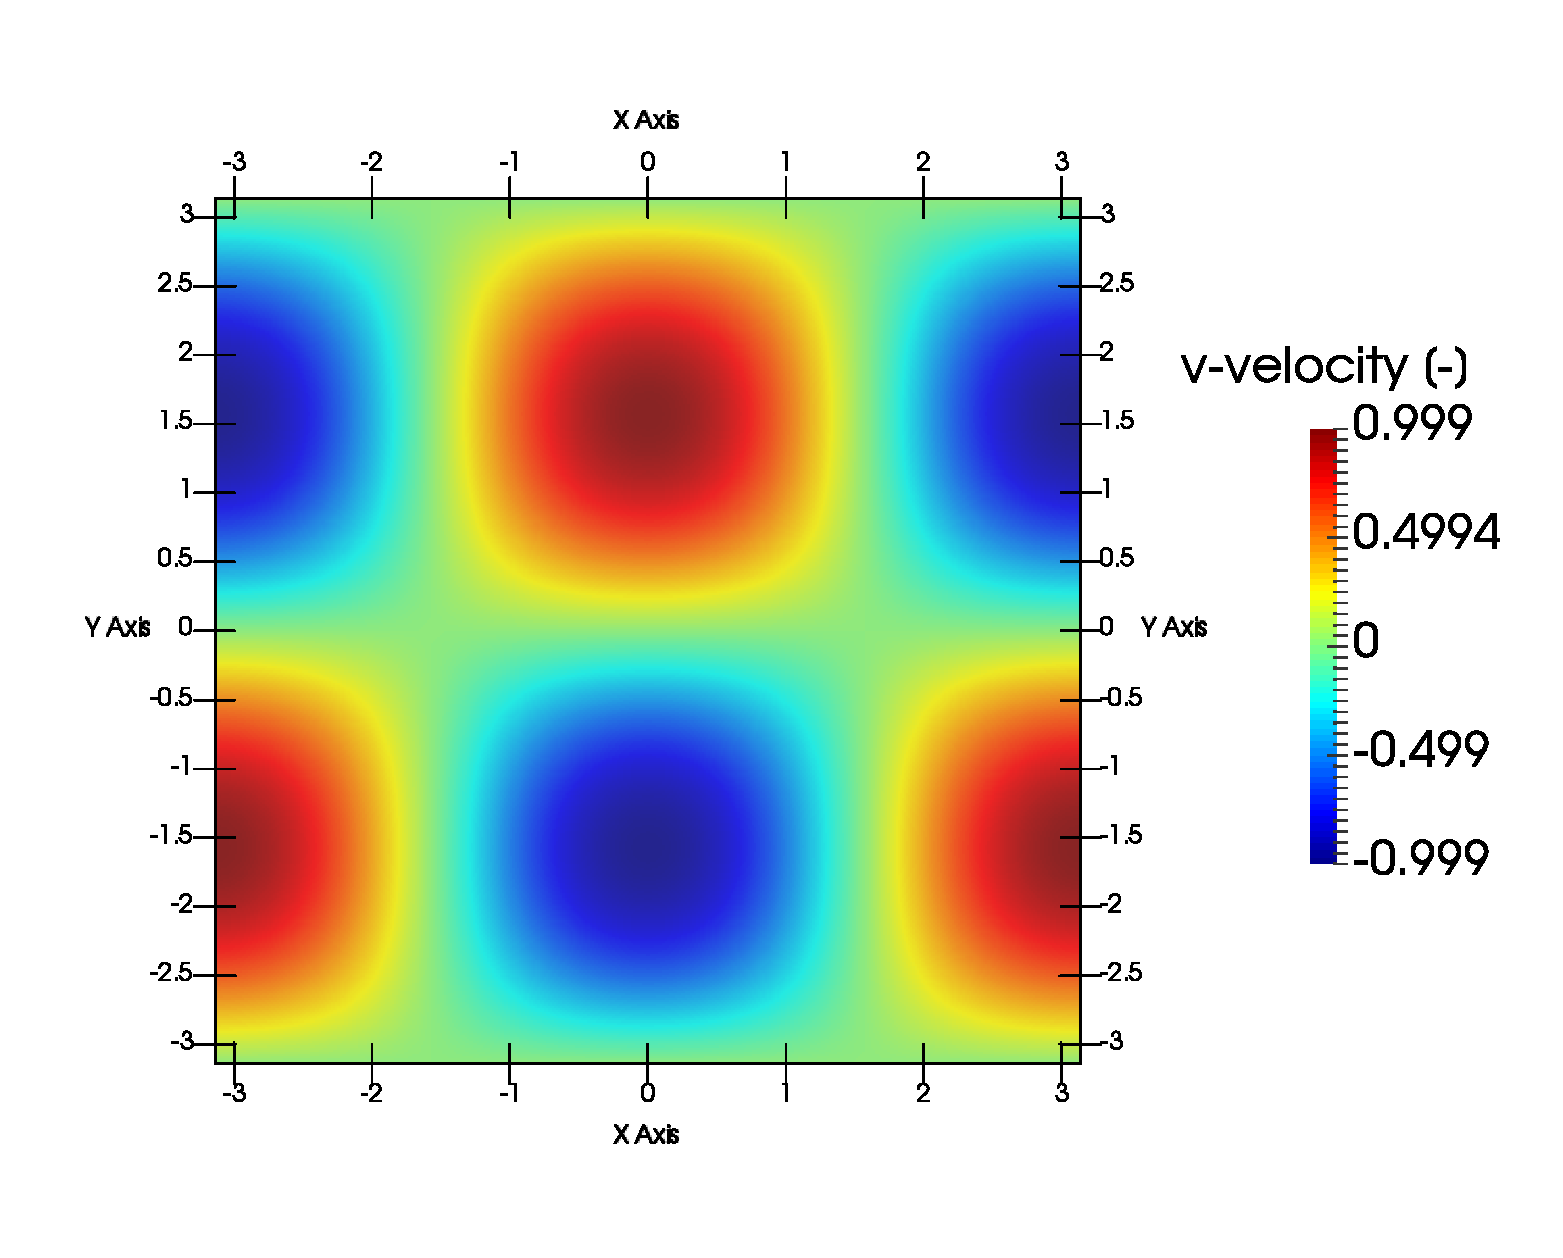
\includegraphics[width=0.48\linewidth]{img/vfield.eps}
       \caption{$u$ and $v$ velocity components on the $z=0$ plane at $t=0$ using the $64^{3}$ elements mesh.}
       \label{f:ic-uv}
\end{figure}


\begin{figure}
 \centering
       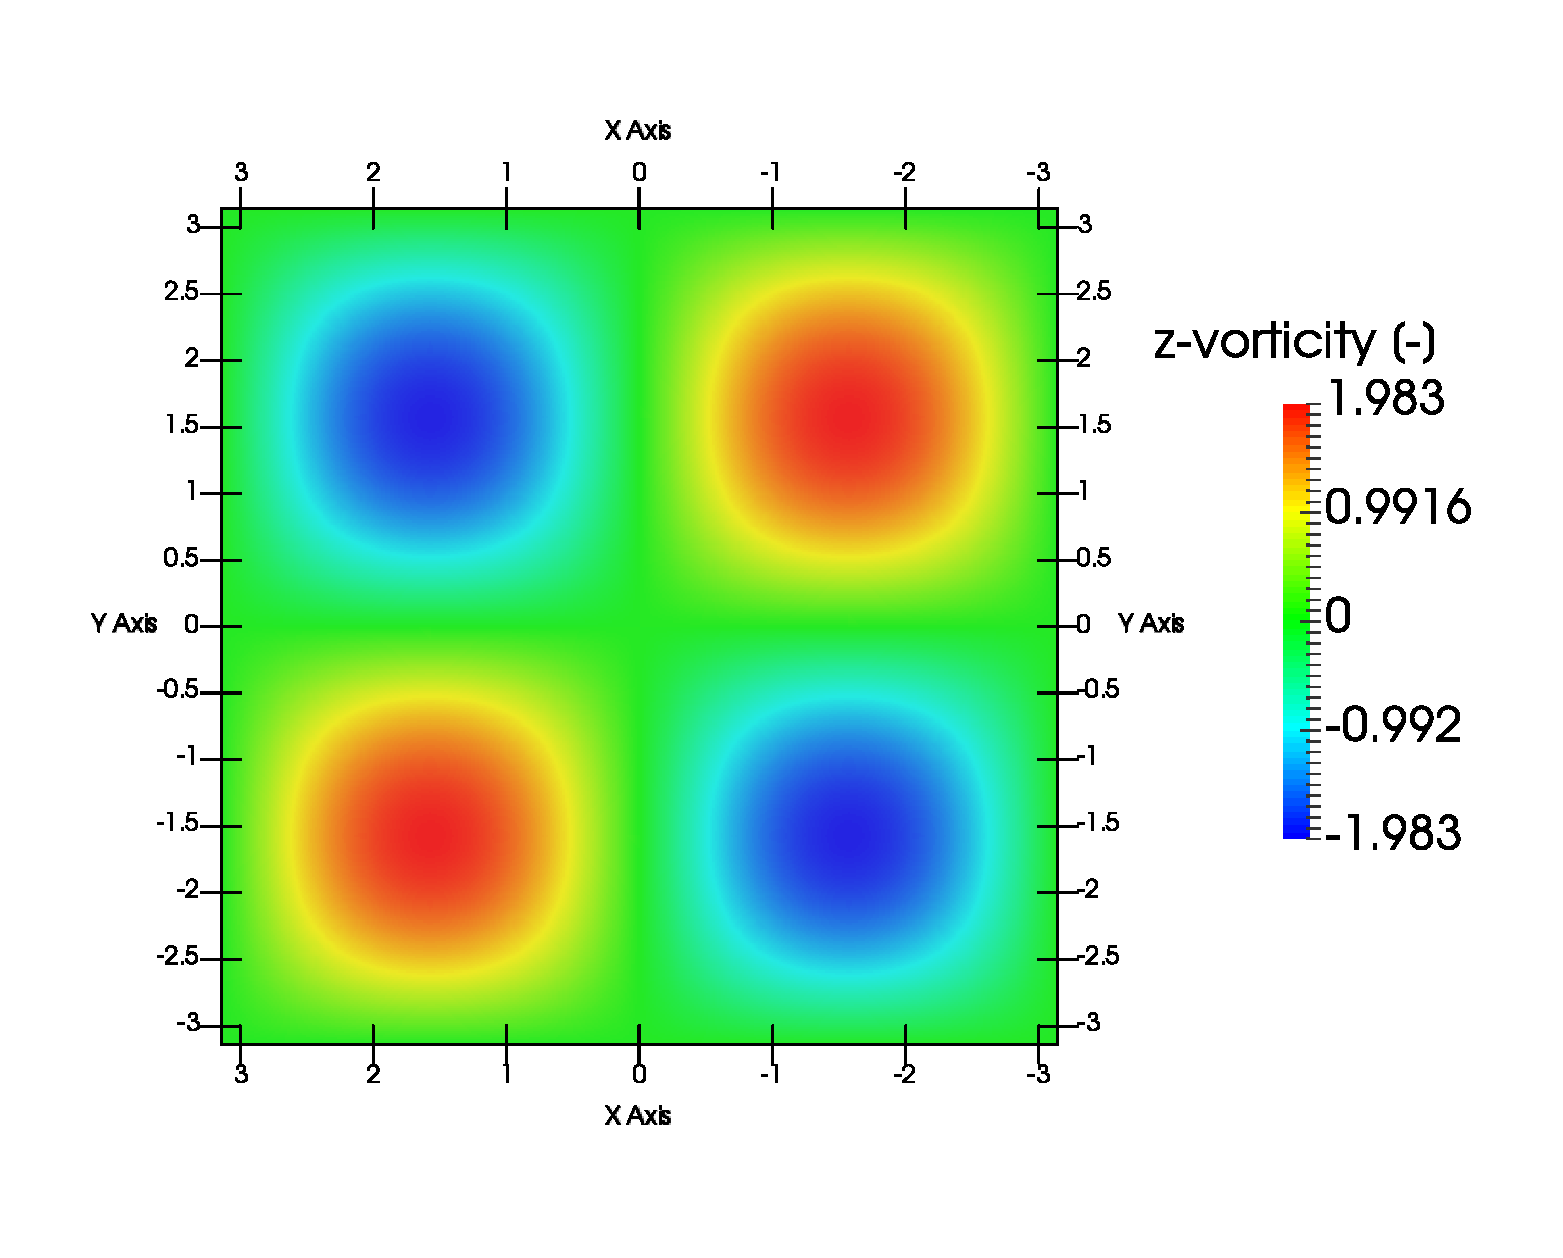
\includegraphics[width=0.48\linewidth]{img/vort.eps}
       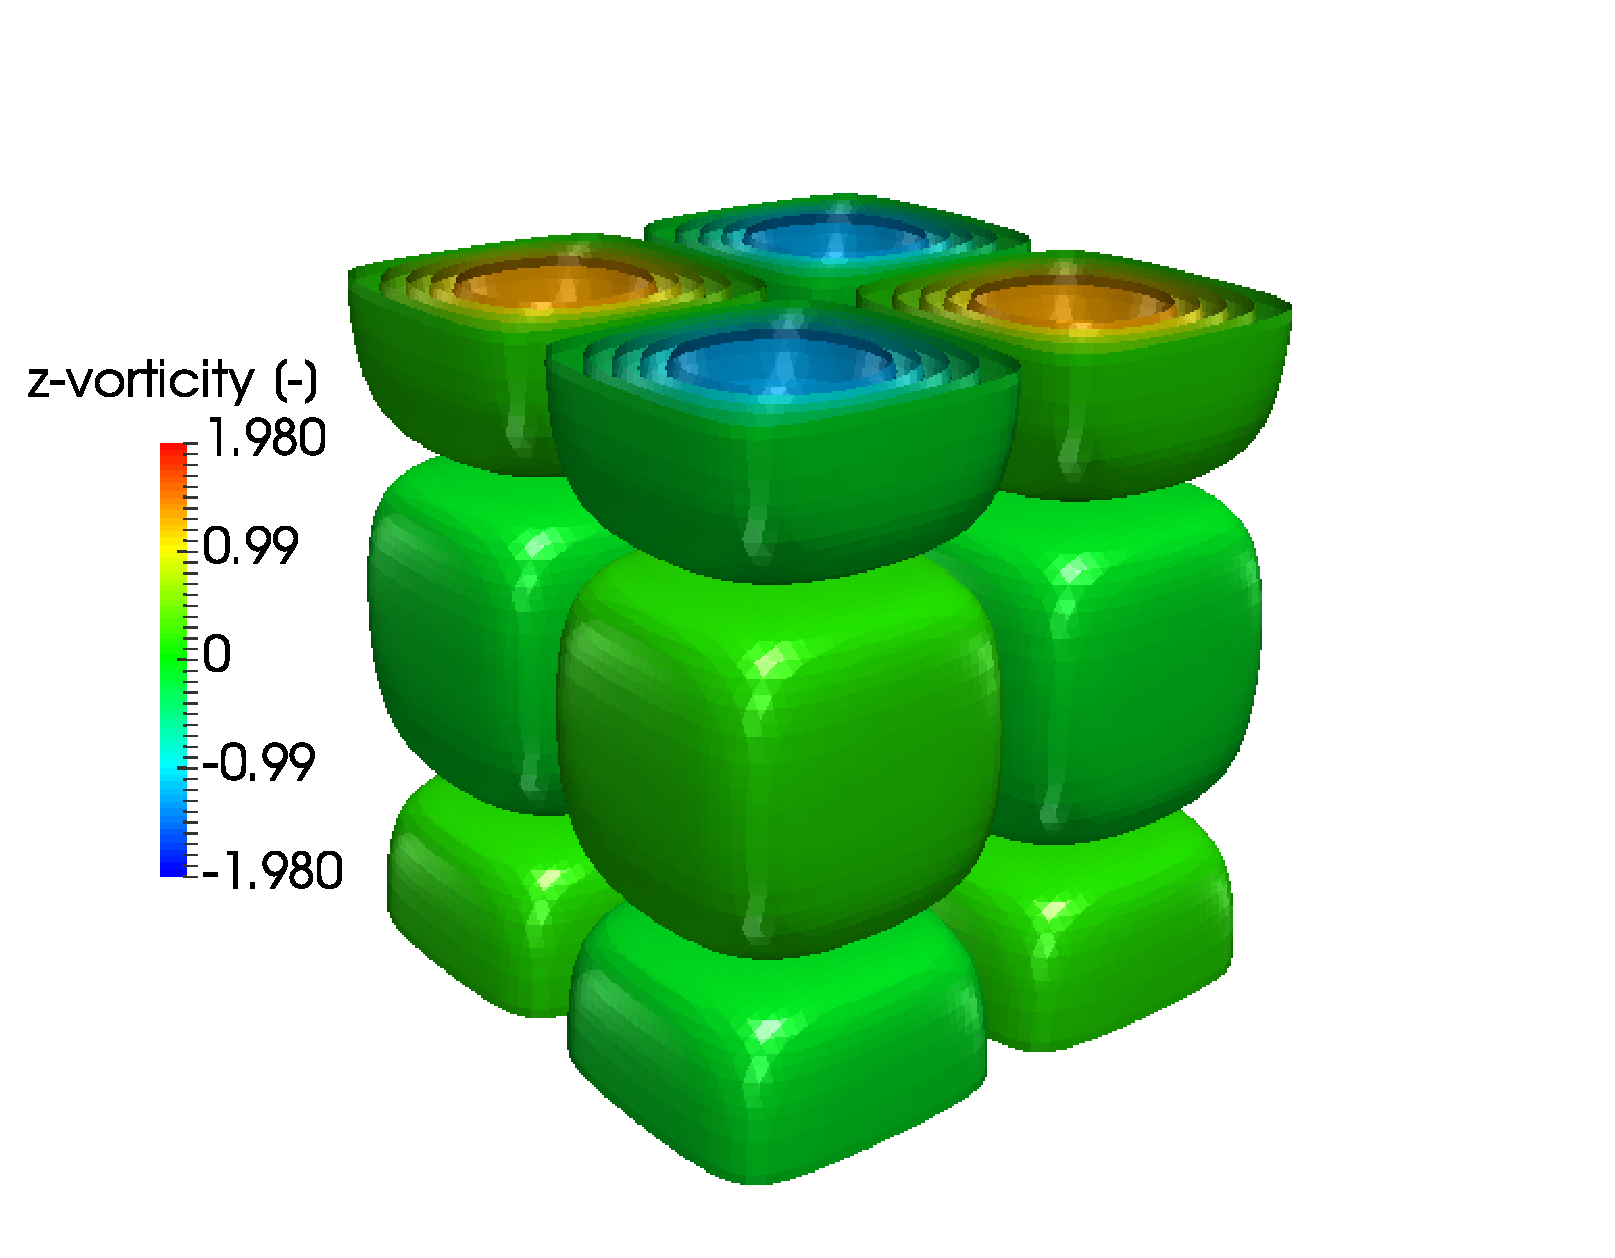
\includegraphics[width=0.48\linewidth]{img/zvort.eps} \\
       \caption{z-vorticity on the surface $z=0$ at $t=0$ and vorticity iso-surfaces at $t=0$ on the $64^3$ volume domain.}
       \label{f:ic-vort}
       \end{figure}

\noindent
The $u$ and $v$ velocity components of the vector field are shown in
Fig~\ref{f:ic-uv}. Note how these fields are formed by contiguous patches of
velocity of same magnitude and opposed direction. The resulting flow, when both
velocity fields are combined, is presented in Fig.~\ref{f:ic-vort} as vorticity contours. The vortical flow is formed by contiguous pairs of counter-rotating vortices, with strength $\Gamma$ and $-\Gamma$.

\chapter{Configuring and Running the Solver}
We will now proceed to set up the \texttt{.xml} file with the solver characteristics and parameters to run the simulation, using the case with $64^{3}$ as guidance. The settings for the $128^{3}$ are very similar, and it will be specified if otherwise.

The files required can be found under the folder
\texttt{\$NEKTUTORIAL/solver64}. The file  \texttt{TGV64\_conditions.xml} must
be modified to set up the solver. Also in the same folder, \texttt{TGV64\_mesh.xml} contains the definition of the mesh and the expansion bases that will be used for the computation. 

\begin{tipbox}
The geometry contained in \texttt{TGV64\_mesh.xml} under the section \inltt{GEOMETRY} is compressed in binary Base64 format. In case the user wants to see its definition, the file must be converted to an uncompressed format by the command:
\tutorialcommand{\$NEK/NekMesh TGV64\_mesh.xml  TGV64\_mesh.xml:xml:uncompress}
\end{tipbox}

The tag \inltt{EXPANSIONS} defines the type of polynomial expansions to be used
on each element, and their order (\texttt{NUMMODES}$=p+1$) as well as the
\texttt{FIELDS} and \texttt{COMPOSITES} to which they are applied (in this case
the whole domain \texttt{C[0]}). 

The following sections all refer to modifications in the file \texttt{TGV64\_conditions.xml}. 


\section*{Parameters}
The TGV case will be run at $Re=1600$ with integral length scale $L=1$ and
initial velocity $V_{0}=1$ so that the kinematic viscosity $\nu=1/1600$. The
temperature field is not included in the computations since it doesn't influence
the dynamics of the fluid. The physical time of the computation is based on the convective time scale $t_{c}=L/V_{0}=1$ and will be $\tau=20t_{c}$, with the first turbulent structures starting to build up at $\tau=8t_{c}=8$. 

\begin{tutorialtask}
In the file \texttt{TGV64\_conditions.xml} under the tag \inltt{PARAMETERS},
define all the flow parameters for the TGV flow  as described above. These are
declared as: \texttt{Re}, \texttt{Kinvis}, \texttt{V0}, \texttt{L} and
\texttt{FinalTime}. Define the number of steps \texttt{NumSteps} as the ratio of
the \texttt{FinalTime} to the time-step \texttt{TimeStep}.
\end{tutorialtask}

These parameters apply for both $64^{3}$ and $128^{3}$. Remember to set the parameters
following the typical XML syntax:

\begin{lstlisting}[style=XMLStyle]
<PARAMETERS>
    <P> [KEY] = [VALUE] </P>
    ...
</PARAMETERS>    
\end{lstlisting}

Note that expressions using a previously defined \inltt{KEY} can be inputted as
a \inltt{VALUE}.

Once the flow parameters have been defined, we must define the discretisation in
the homogeneous z-direction. Since we are interested in determining the flow on
a cubic mesh, the length of the domain along the z-direction will also be
$L_{z}=2\pi$ (not to be confused with the integral length scale, $L$). We must
also specify the number of Fourier planes we are going to discretise our
z-direction into. For a fully uniform mesh, we then choose $N_{z}=64$ or $128$,
depending on the case that we are running. This corresponds to $32$ or $64$
complex Fourier modes, respectively.

Additionally, we also enable the spectral vanishing viscosity (SVV) feature
which acts to dampen high-frequency oscillations in the solution which would
otherwise introduce numerical instability.

\begin{tutorialtask}
In the file \texttt{TGV64\_conditions.xml} under the tag \inltt{PARAMETERS}, define all the solver parameters for the homogeneous z-direction discretisation as described above. These include: 
\begin{itemize}
\item \texttt{LZ} and \texttt{HomModesZ}. 
\item The SVV diffusion coefficient \texttt{SVVDiffCoeff} set to 0.1 and the Fourier cut-off frequency ratio \texttt{SVVCutoffRatio} set to 0.7
\end{itemize}

\end{tutorialtask}

These parameters also apply for both $64^{3}$ and $128^{3}$, except for $N_{z}$ which
must be set to $128$ instead for the latter case. Note that $\pi$ can be used directly
with the keyword \inltt{PI}.


\section*{Solver Properties}
We now declare how the flow will be solved. We will use the Velocity Correction
Scheme (VCS) to solve the components of the unsteady Navier-Stokes equations
separately, rather than as one single system. We must also specify the time
integration method, which will be explicit-implicit of order 2, and the
approach to be used when solving linear matrix systems of the form $Ax=b$ that arise from the VCS scheme. Finally, we must describe how the homogeneous z-direction will be treated in the quasi 3D approach. 

\begin{tutorialtask}
In the file \texttt{TGV64\_conditions.xml} under the tag \inltt{SOLVERINFO}, define all the solver properties. These include:
\begin{itemize}
\item Setting the \texttt{TimeIntegrationMethod} to \texttt{IMEXOrder2}. 
\item Setting the \texttt{SolverType} to \texttt{VelocityCorrectionScheme} and the \texttt{EqType} to \texttt{UnsteadyNavierStokes}.
\item (Optional) Setting the \texttt{UseFFT} property to \texttt{True} to indicate that the
    Fast Fourier Transform method will be used to speed up the operations
        related to the harmonic expansions, using the FFTW library.
		This may only be used if sources have been compiled with the
		CMake option \inltt{NEKTAR\_USE\_FFTW} set to \texttt{ON} or
		if you are using a binary package.
\item Setting \texttt{Homogeneous} to \texttt{1D} to tell the solver we are
    using harmonic expansions along the z-direction only.
\item Setting \texttt{GlobalSysSoln} to \texttt{DirectMultiLevelStaticCond} to
    specify that a serial Cholesky factorisation will be used to directly solve the global linear systems.
\item Setting the properties \texttt{SpectralHPDealiasing} and \texttt{SpectralVanishingViscosity} both to \texttt{True}.

\end{itemize}
\end{tutorialtask}

These properties apply for both $64^{3}$ and $128^{3}$ cases. Remember to set the
property/value pairs following the typical XML syntax:

\begin{lstlisting}[style=XMLStyle]
<SOLVERINFO>
    <I PROPERTY="[STRING]" VALUE="[STRING]" />
    ...
</SOLVERINFO>    
\end{lstlisting}

\section*{Boundary and Initial Conditions}
The periodic boundary conditions for the domain are already defined for the user in the \texttt{.xml} file, under the tag \inltt{BOUNDARYCONDITIONS}. The initial conditions can be prescribed to the solver by means of a standard function. 

\begin{tutorialtask}
In the file \texttt{TGV64\_conditions.xml}, within the \inltt{CONDITIONS}
    section, create a function named \texttt{InitialConditions} where the
    initial conditions for the variables \texttt{u,  v, w} and \texttt{P} are
    defined. Go back to Chapter 1 if you don't remember the expressions for the
    initial conditions.

\end{tutorialtask}

Multi-variable functions such as initial conditions and analytic
solutions may be specified for use in, or comparison with, simulations. These
may be specified using expressions (\inltt{<E>})

\begin{lstlisting}[style=XMLStyle]
<FUNCTION NAME="[NAME]">
    <E VAR="[VARIABLE_1]" VALUE="[EXPRESSION]"/>
    <E VAR="[VARIABLE_2]" VALUE="[EXPRESSION]"/>
    ...
</FUNCTION>
\end{lstlisting}

\section*{Filters}
Turbulent flows, as is the TGV flow, have very high diffusivity. The random and chaotic motion of the fluid particles results in an increased momentum and mass convection as well as heat transfer, with the flow composed of fluid structures with a wide range of length scales. The large, energy-containing fluid structures inertially break down into smaller and smaller structures by vortex stretching, with an associated kinetic energy transfer between the scales. When these small fluid structures are of the size of the Kolgomorov length scales $\eta$, molecular viscosity becomes substantial and dissipates the kinetic energy into heat. As such, a good way of characterising turbulent flows is via the evolution of the kinetic energy or, more appropriately, via its dissipation rate.
 
\begin{tutorialtask}
In the file \texttt{TGV64\_conditions.xml}, within the \inltt{FILTERS} section, create two filters:
\begin{itemize}
\item A \texttt{ModalEnergy}-type filter named \texttt{TGV64MEnergy} which will compute the energy spectrum of the flow. Set its \texttt{OutputFrequency} to 10 timesteps.
\item A second, \texttt{Energy}-type filter named \texttt{TGV64Energy}, which will calculate the time evolution of the kinetic energy and the enstrophy. Set its \texttt{OutputFrequency} to 10 timesteps. 
\end{itemize}
\end{tutorialtask}

\begin{lstlisting}[style=XMLStyle]
<FILTER TYPE="TypeName">
    <PARAM NAME="OutputFile">FileName</PARAM>
    <PARAM NAME="OutputFrequency">10</PARAM>
</FILTER>
\end{lstlisting}
 
\section*{Running the Solver}
If you have not completed \texttt{Task 1.2} or would like to test your configuration,
the \texttt{IncNavierStokesSolver} can now be run with the XML files above to
solve the TGV problem.

\begin{tutorialtask}
Run the solver by typing the following command on the command line:
\tutorialcommand{\$NEK/IncNavierStokesSolver TGV64\_mesh.xml TGV64\_conditions.xml}
\end{tutorialtask}

\begin{tipbox}
    To reduce the solution time on computers with multi-core, or multiple,
    processors, MPI can be used to run the simulation in parallel. Note that,
	for binaries compiled from source, the CMake option \inltt{NEKTAR\_USE\_MPI}
	must have been set to \texttt{ON}. To run in parallel,
    prefix the command in the previous task with \texttt{mpirun -np X},
    replacing \texttt{X} by the number of parallel processes to use. For
    example, to use two processes:

    \tutorialcommand{mpirun -np 2 \$NEK/IncNavierStokesSolver TGV64\_mesh.xml  TGV64\_conditions.xml}
	
	Additionally, setting \texttt{GlobalSysSoln} to \texttt{XxtMultiLevelStaticCond}
	(\texttt{Task 3.3}) will specify that a \textit{parallel} Cholesky factorisation will be used to
	directly solve the global linear systems using the $XX^{T}$ library.
\end{tipbox}


\chapter{Simulation Results}
You will now have to post-process the files in order to see the results of the simulation. You may either use output files of your recent run or those provided in the folder \texttt{completed/solver64}. Amongst the output files, you can find the checkpoint files \texttt{.chk} and final file \texttt{.fld} that contain the state of the simulation at each time step; the modal energy file \texttt{.mdl} containing the energy spectrum of the Fourier modes; and the energy file \texttt{.eny} with the evolution of the kinetic energy and the enstrophy. Note that the folder \texttt{completed/solver64} does not contain \texttt{.chk} files.

Both energy files are easily post-processed and can be converted to the MATLAB
readable format \texttt{.dat}, just by changing the file extension. The
checkpoint files however, must be converted to a standard visualisation
data format so that they are readable with Paraview or other visualisation software. 

\begin{tutorialtask}
In the folder \texttt{solver64}, which contains the checkpoint files, type the command:
\tutorialcommand{\$NEK/FieldConvert -m vorticity TGV64\_mesh.xml
    TGV64\_mesh\_0.chk TGV64\_mesh\_0.vtu}
This command will convert the file to the VTK visualisation format and will also
calculate the vorticity throughout the volume. Note that it only converts
one checkpoint file at a time. A shell script could be used to convert as many
files as desired. This command may also be used on the \texttt{.fld} file.
\end{tutorialtask}

The evolution of the kinetic energy of the flow is obtained by integrating the square of the velocity norm over the domain. Similarly, the enstrophy is calculated by integrating the square of the vorticity norm over the domain:
\vspace{0.1 cm}
\begin{equation}
E_{k}=\frac{1}{2\mu(\Omega)}\int_{\Omega}\|\textbf{u}\|^{2}dx \hspace{3 cm}
\zeta = \frac{1}{2\mu(\Omega)}\int_{\Omega}\|\omega\|^{2}dx
\end{equation}
 
The enstrophy is a measure of the intensity of the vorticity and is related to
dissipation effects of the flow. More precisely, under the assumption of
incompressible flow, the enstrophy is related to the kinetic energy dissipation
rate, $\epsilon$, via the equation on the left. It is also defined as the rate of change of the kinetic energy, the equation on the right:
\vspace{0.1 cm}
\begin{equation}
\epsilon=2\nu \zeta \hspace{3 cm} \epsilon=-\frac{dE_{k}}{dt}
\end{equation}
\vspace{0.1 cm}Therefore, the dissipation rate can be calculated both from the
enstrophy and numerically from the evolution of the kinetic energy. From the
modal energy file, it is possible to evaluate the energy spectrum of the Fourier modes. This will in turn be helpful to identify what length scales carry the most energy. After post-processing the energy files on MATLAB, you should be able to produce the following figures, which depict the time evolution of the kinetic energy and enstrophy of the flow, as well as the evolution of the dissipation rate (both computed and enstrophy-based) and the energy spectrum: 

\begin{figure}[h!]
 \centering
   \begin{tabular}{cc}
       \includegraphics[width=0.5\linewidth]{img/Ek.eps}
       \includegraphics[width=0.5\linewidth]{img/enstrophy.eps} \\
       \end{tabular}
       \label{fig:fig1}
       \caption{Time evolution of the kinetic energy (left) and enstrophy (right).}
       \end{figure}

\begin{figure}[h!]
 \centering
   \begin{tabular}{cc}
       \includegraphics[width=0.5\linewidth]{img/epsilon.eps}
       \includegraphics[width=0.5\linewidth]{img/Fourier_E.eps} \\
       \end{tabular}
       \label{fig:fig1}
       \caption{Time evolution of numerically computed and enstrophy-based dissipation rates (left) and time evolution of the energy spectrum of the fourier modes (right).}
       \end{figure}
       
\begin{tipbox}

The data may be plotted using the freely available gnuplot package, widely available on Linux systems. Example gnuplot files are provided in the folders \texttt{completed/solver64} and \texttt{completed/solver164}. Such files can be run with the simple command:
\tutorialcommand{gnuplot TGV64Energy.gnuplot}

\end{tipbox}

The time evolution of the kinetic energy is well predicted by the spectral, quasi-3D computation. Since no force is applied to the fluid, the initial kinetic energy in the flow is progressively dissipated, with the dissipation rate peaking at around $\tau\approx 9$ when the turbulent fluid structures are formed. This is consistent with the enstrophy. The enstrophy, which is a measure of how vortical the flow is, peaks at the same time as the dissipation rate, $\tau\approx 9$: vortex stretching increases vorticity in the stretching direction and reduces the length scale of the fluid structures. Hence, when vorticity is at its highest, the flow is dominated by these small structures, which are responsible for the main viscous dissipation effects. The discrepancy between the numerically computed and enstrophy-based dissipation rates is directly related to the resolution of the mesh. The enstrophy-based dissipation rate being lower than the numerically calculated one means that, in the simulation, not all of the dissipation is due to the vorticity present in the flow. The low resolution of the mesh accentuates the numerical diffusion present in the spectral/\textit{$hp$} element method and is the reason for the discrepancy.

Finally, from the evolution of the energy spectrum of the Fourier modes it is possible to infer how the flow behaves. Initially, all the energy is contained in the smallest wavenumbers, meaning that the flow is dominated by the large length scales. As time passes, the energy is progressively transferred to smaller and smaller scales (larger wavenumber). This energy in the small scales peaks between $\tau=8$ and $\tau=10$, when the flow is fully turbulent, and then dies out for all wavenumbers due to dissipation. This process is depicted in the figures below, through the z-component of the vorticity.

\begin{figure}
\begin{subfigure}{0.32\textwidth}
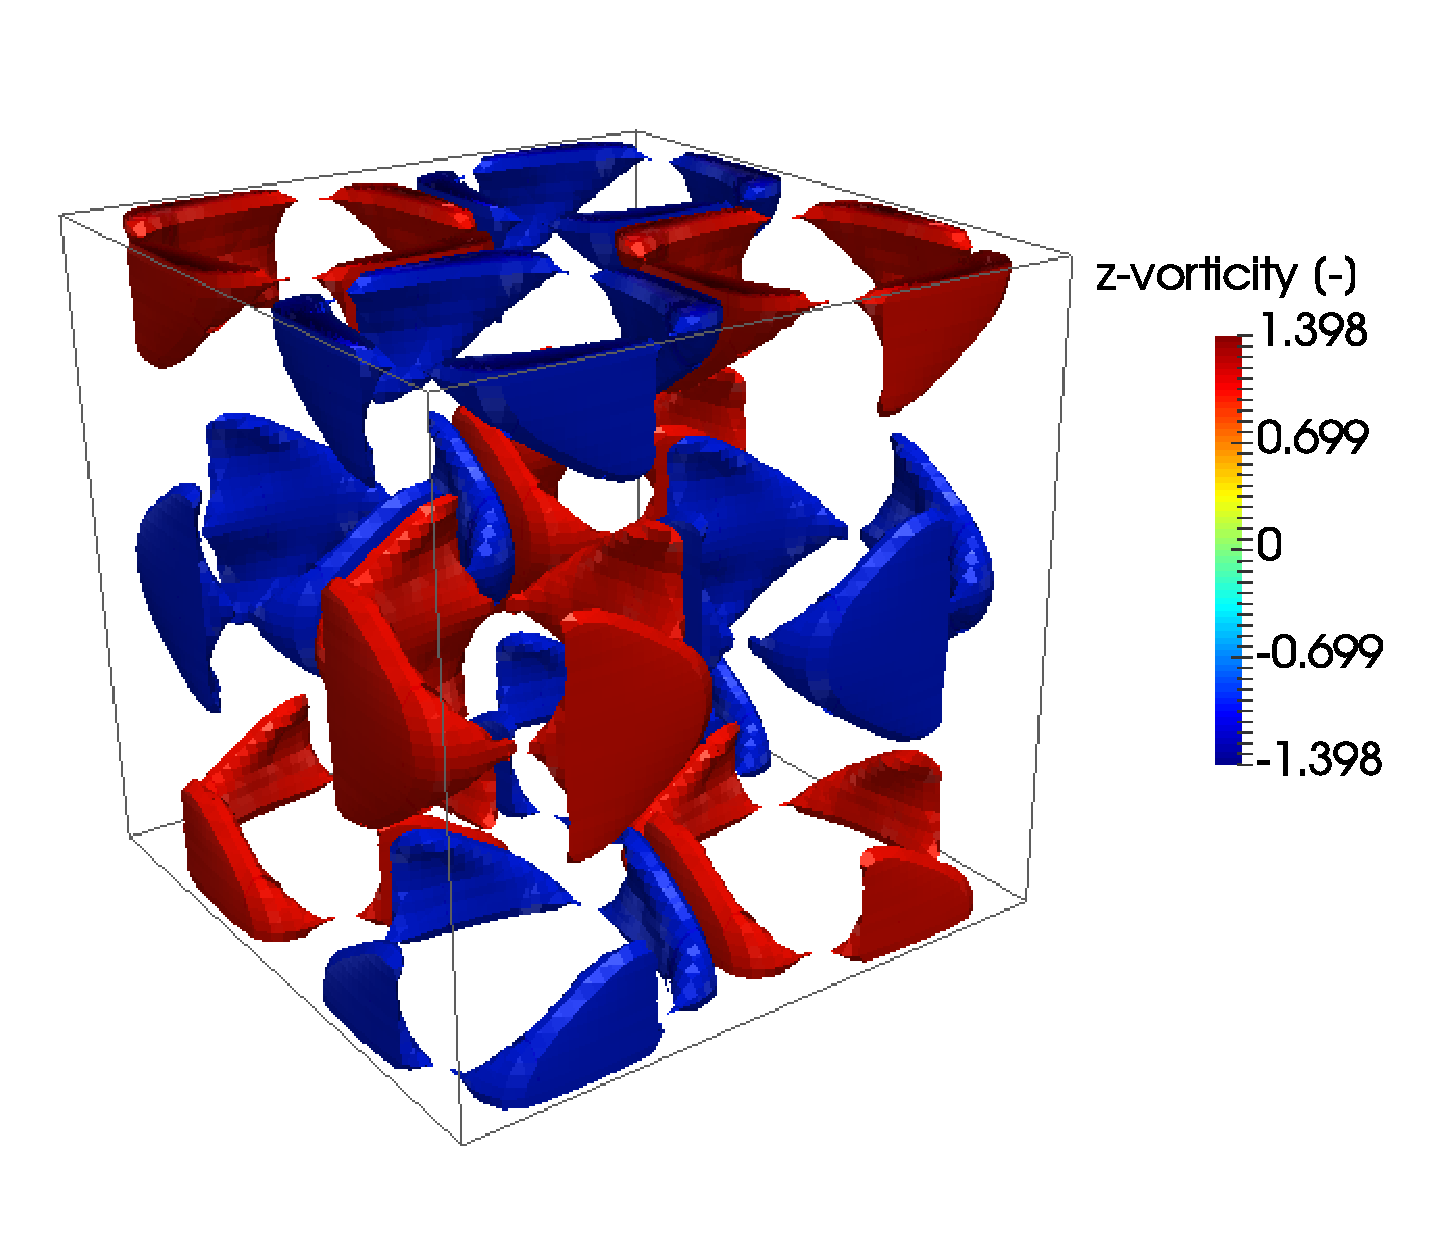
\includegraphics[width=\linewidth]{img/t3.eps}
\caption{$\tau$=3, Laminar vortex sheets} \label{fig:1a}
\end{subfigure}
\begin{subfigure}{0.32\textwidth}
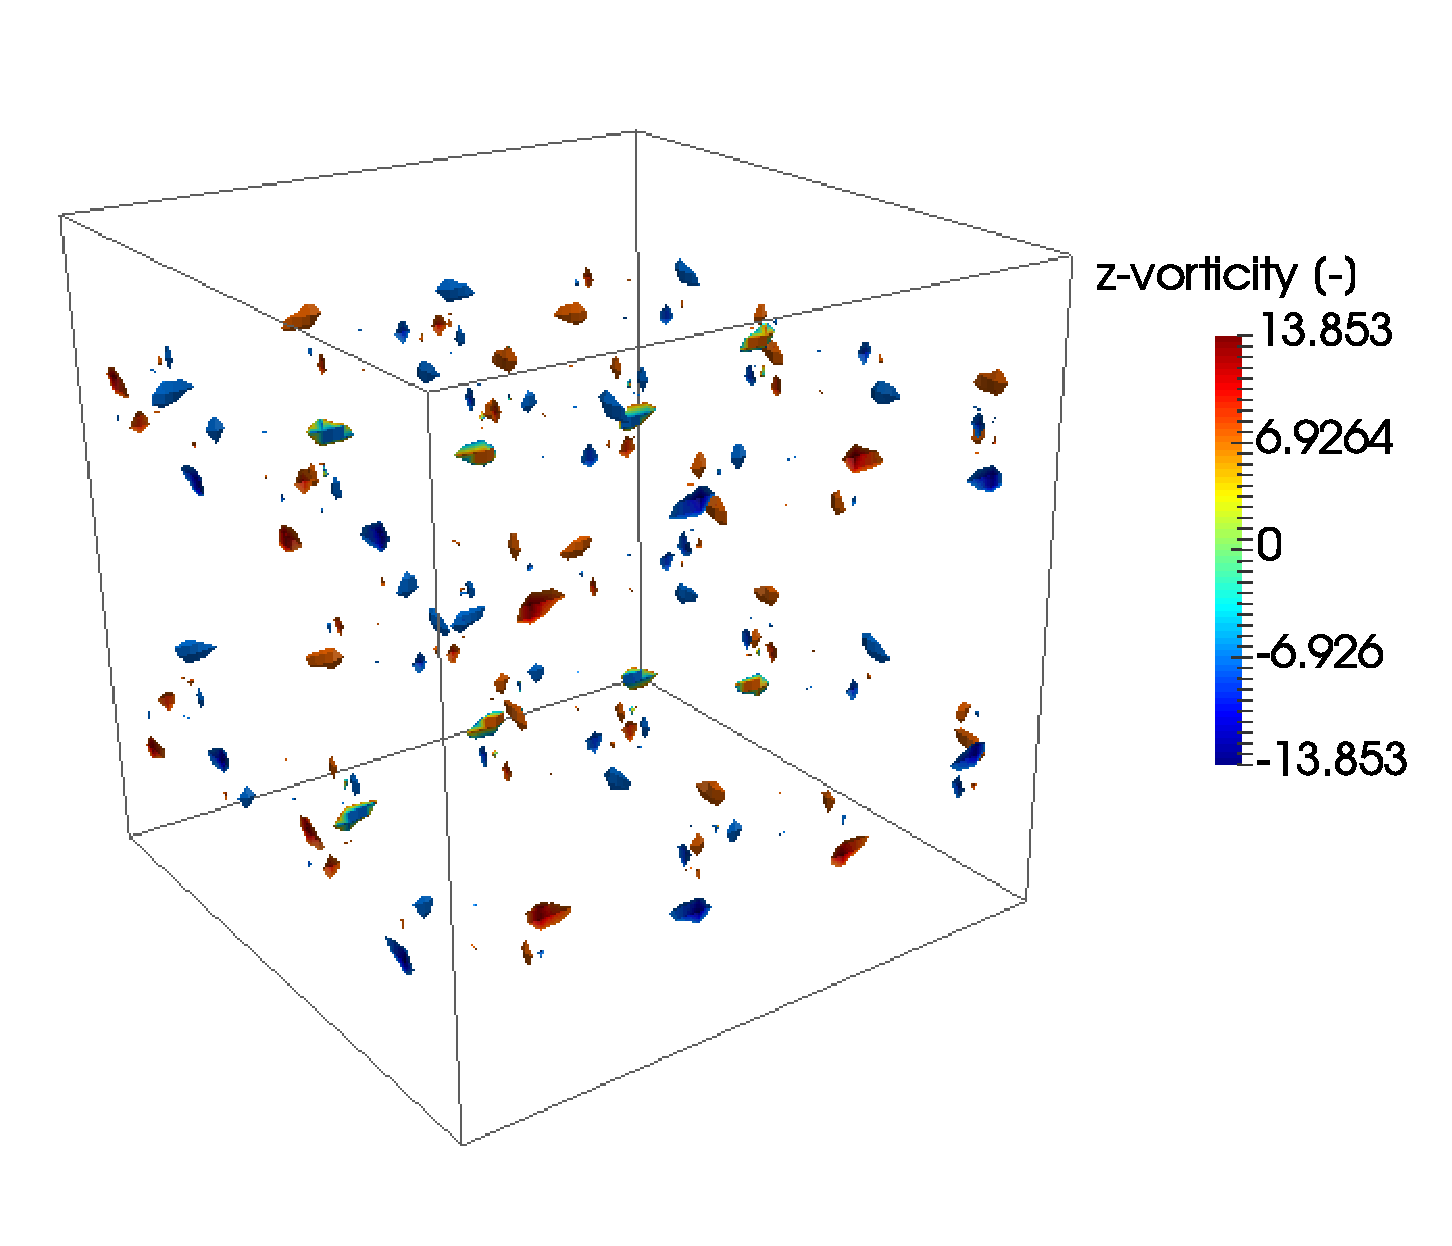
\includegraphics[width=\linewidth]{img/t5.eps}
\caption{$\tau$=5, Vortex stretching} \label{fig:1b}
\end{subfigure}
\begin{subfigure}{0.32\textwidth}
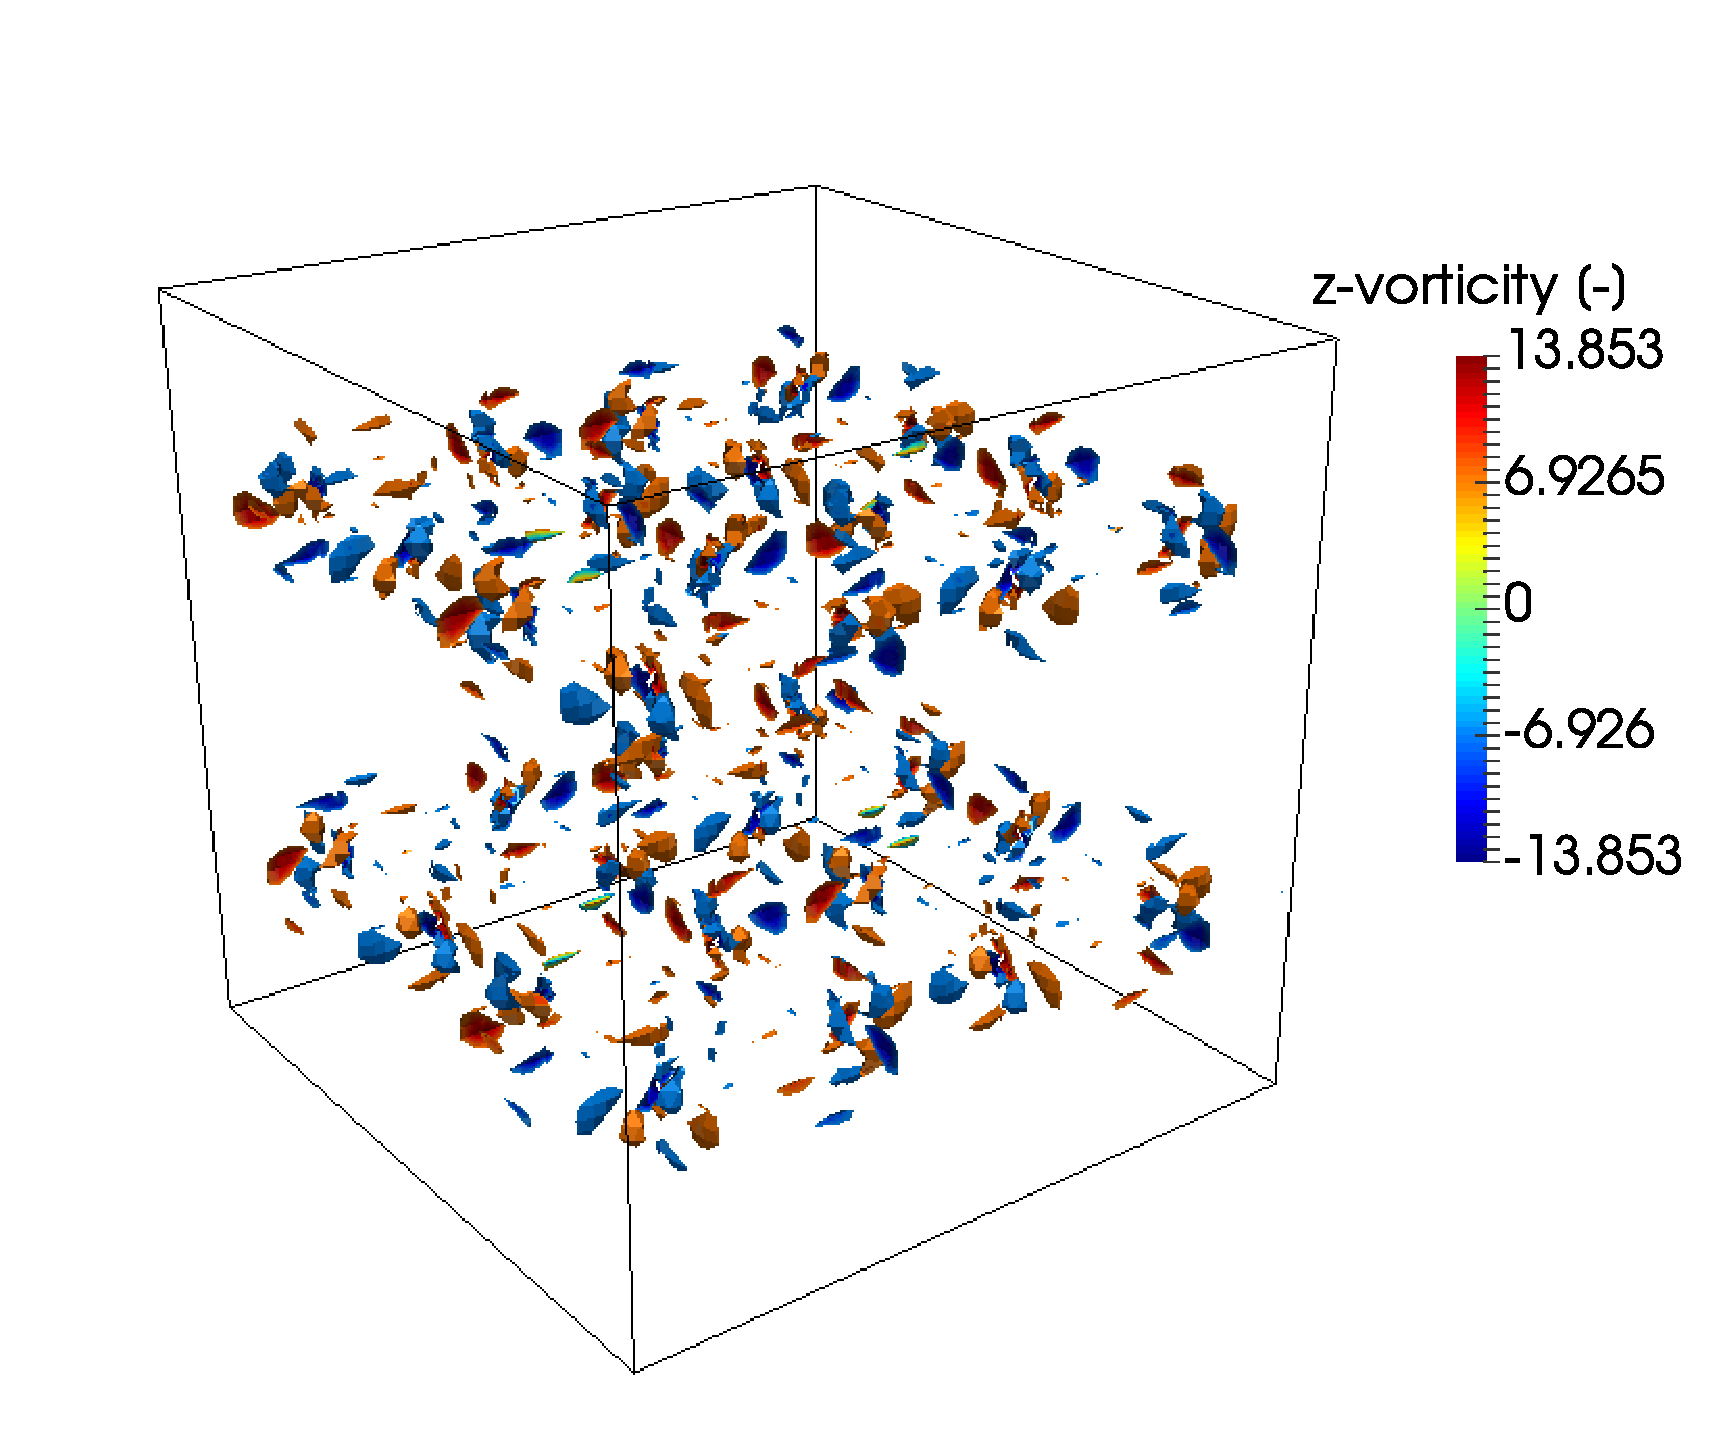
\includegraphics[width=\linewidth]{img/t7.eps}
\caption{$\tau$=7, Rearrangement} \label{fig:1c}
\end{subfigure}
\begin{subfigure}{0.32\textwidth}
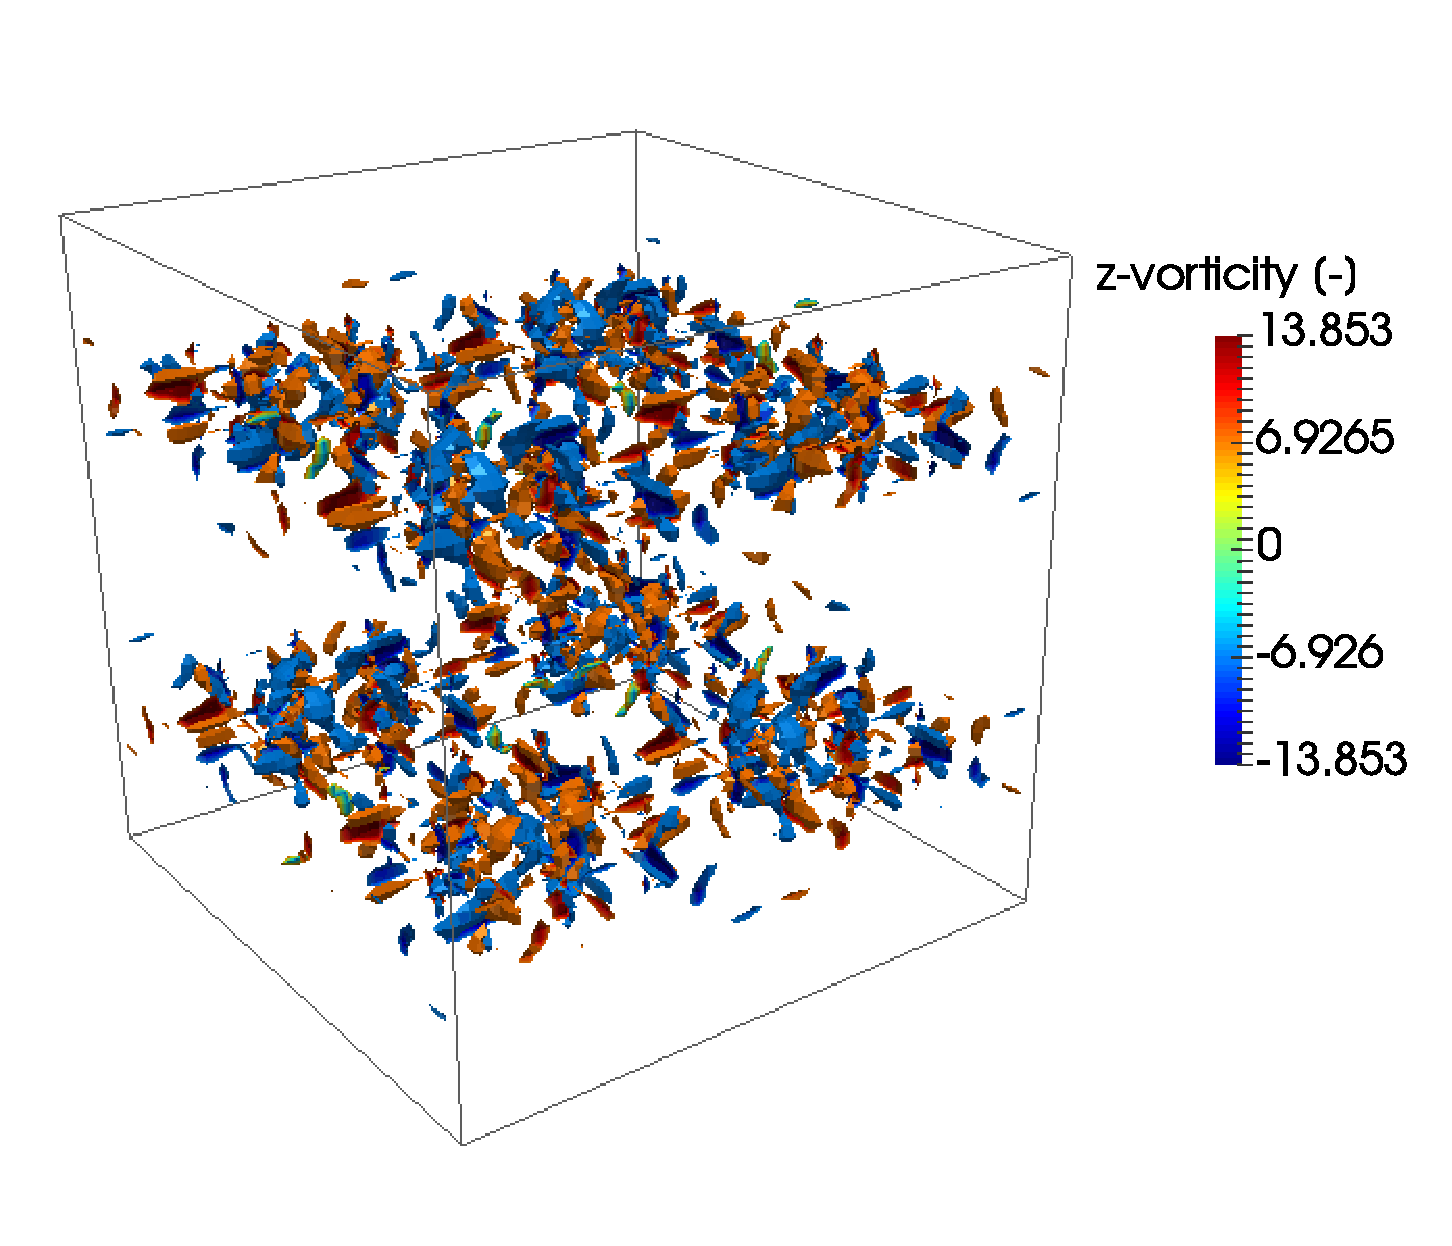
\includegraphics[width=\linewidth]{img/t8.eps}
\caption{$\tau$=8, Breakdown} \label{fig:1c}
\end{subfigure}
\begin{subfigure}{0.32\textwidth}
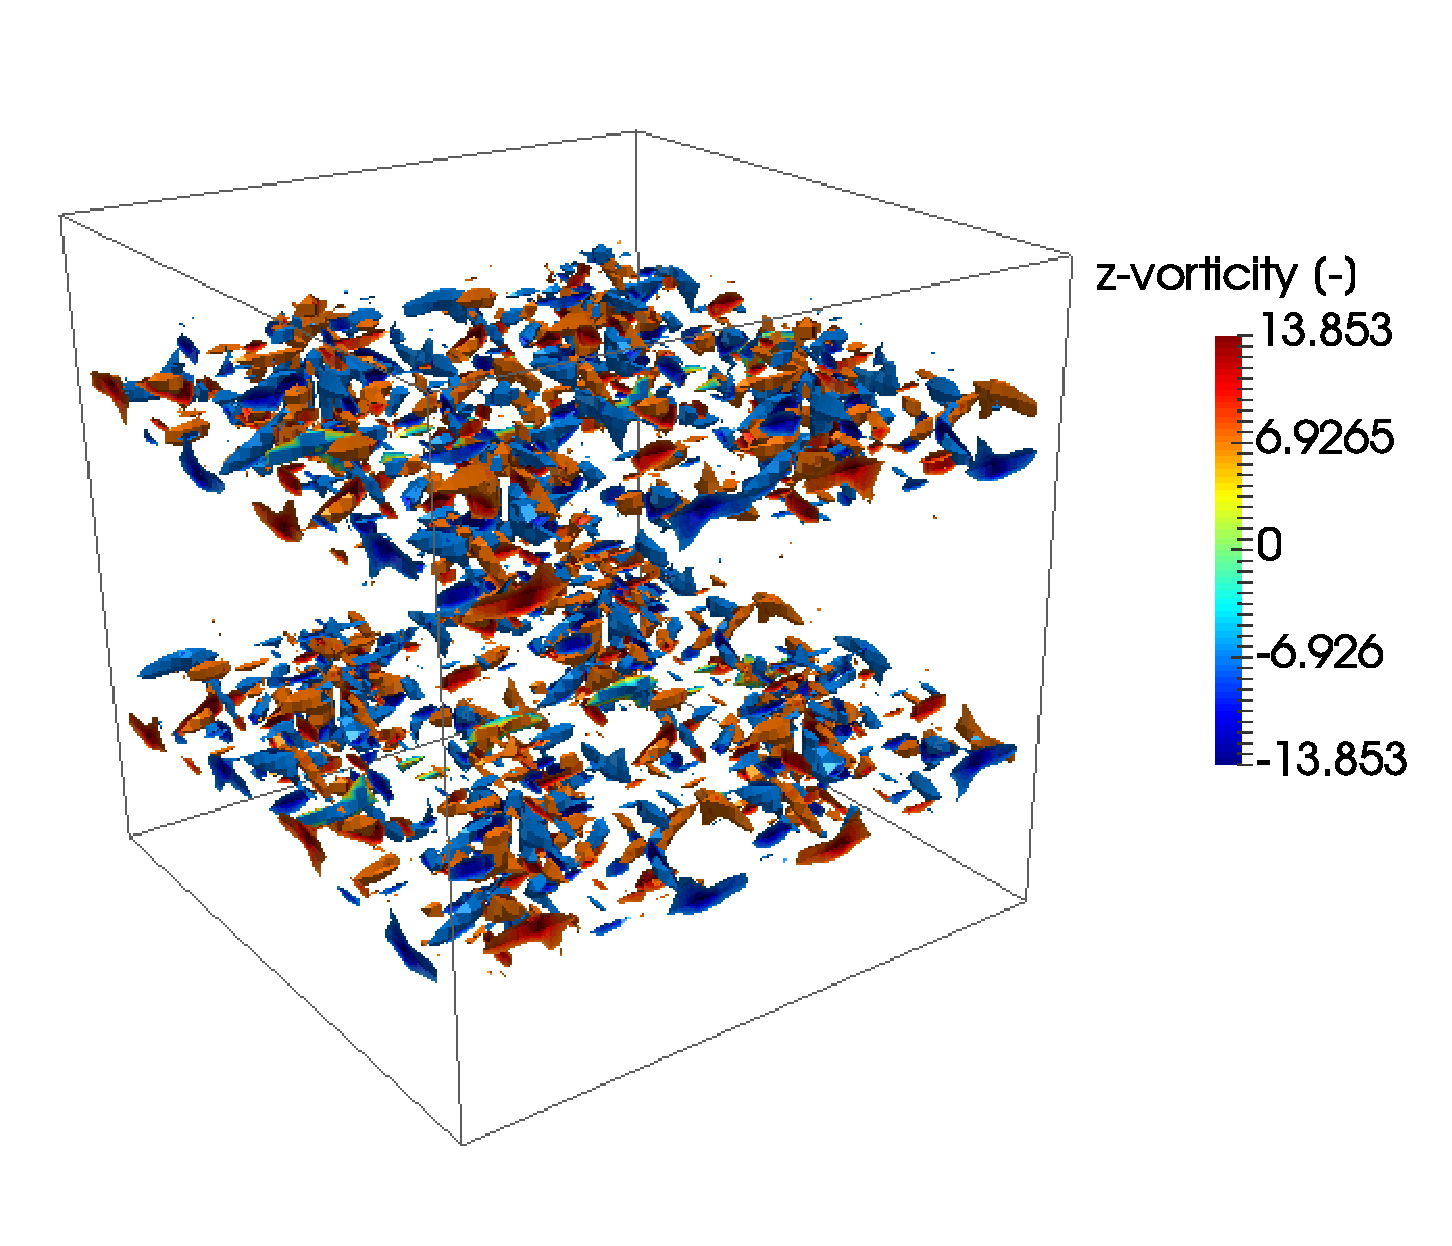
\includegraphics[width=\linewidth]{img/t9.eps}
\caption{$\tau$=9, Fully turbulent} \label{fig:1c}
\end{subfigure}
\begin{subfigure}{0.32\textwidth}
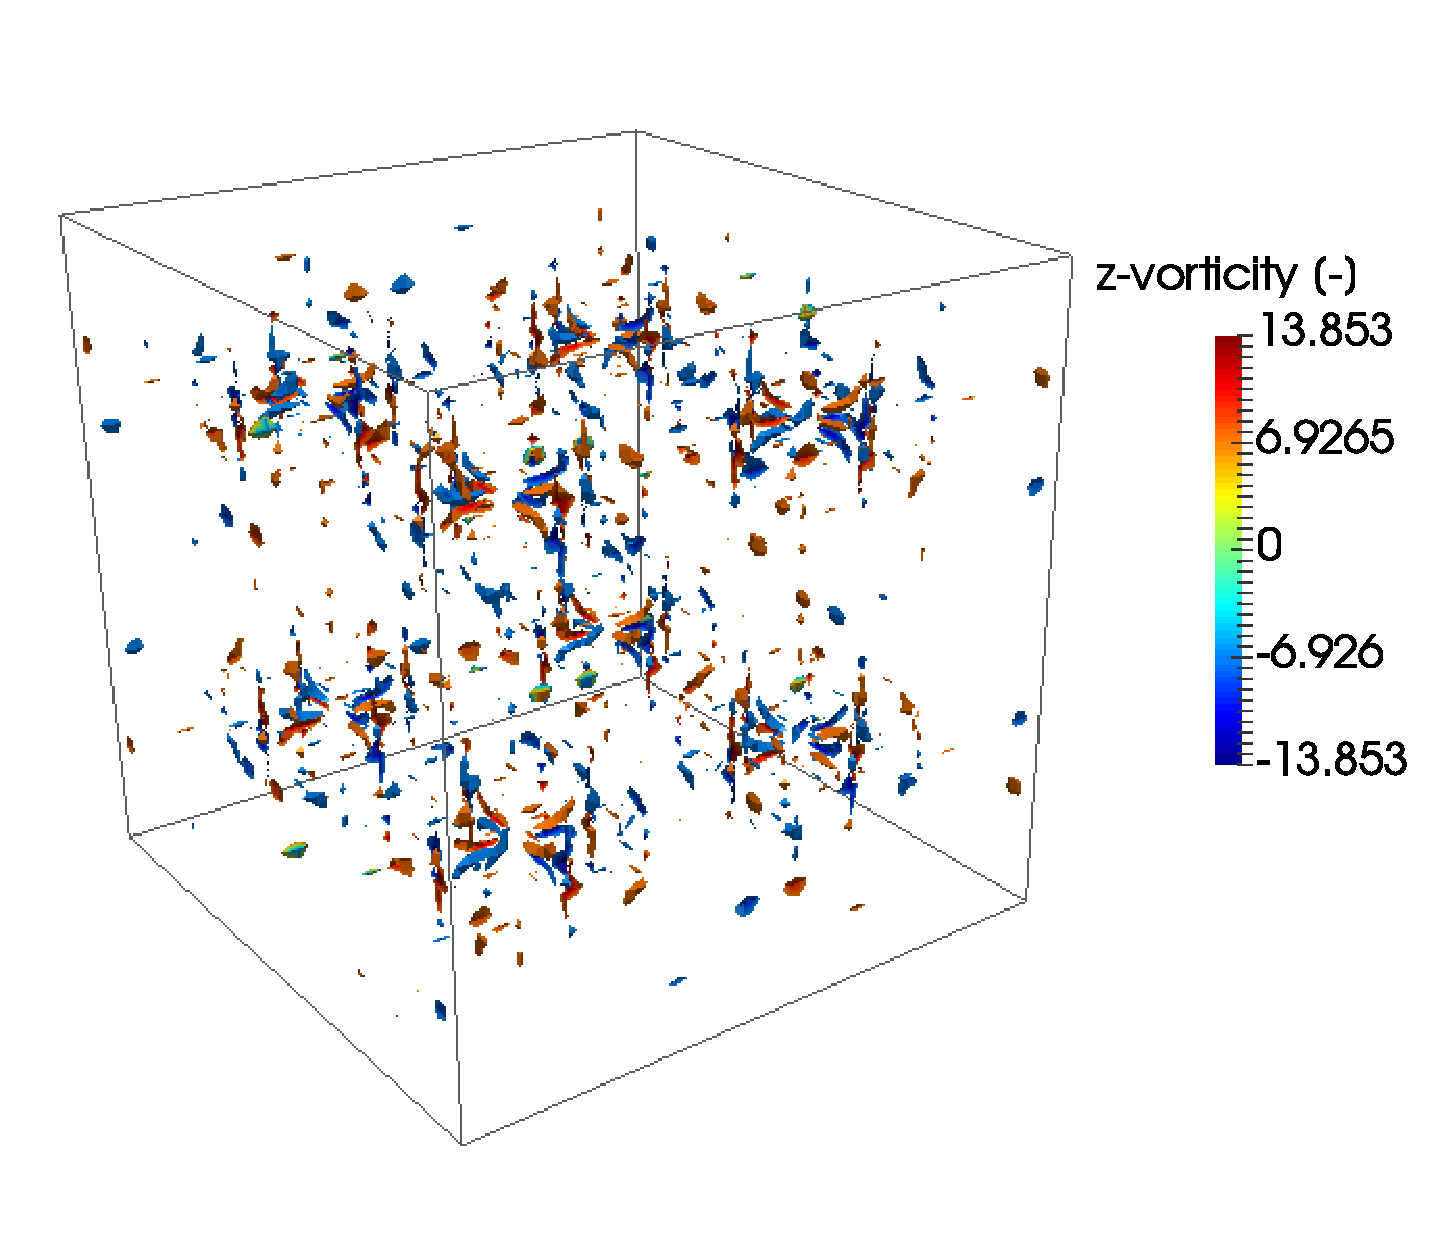
\includegraphics[width=\linewidth]{img/t12.eps}
\caption{$\tau$=12, Dissipation and decay} \label{fig:1c}
\end{subfigure}
\caption{Time evolution of z-vorticity isosurfaces} \label{fig:1}
\end{figure}
 

\begin{advancedtutorialtask}
Running the simulation with a mesh of $128^{3}$ is a bit more computationally expensive and it is left as an optional exercise. If you do run this simulation, extract the information from the energy files and plot the time evolution of the kinetic energy, enstrophy and dissipation rate for both cases under the same graphs. Establish a qualitative and quantitave comparison between the results of using different resolutions to resolve the Taylor-Green Vortex flow.
\end{advancedtutorialtask}



\begin{center}
\textbf{\Large This completes the tutorial.}
\end{center}



\end{document}
